\documentclass[12pt]{article}
\PassOptionsToPackage{quiet}{fontspec}
\usepackage[a4paper]{geometry}
\geometry{a4paper,left=1in,right=1in,top=1.5in,bottom=1in}
\usepackage{fancyhdr}
\pagestyle{fancy}
\setlength{\headheight}{1.5em}
\renewcommand{\headrulewidth}{2pt}
\usepackage{amsmath}
\usepackage{amsfonts}
\usepackage{bm}
\usepackage{enumerate}
\usepackage{xfp}
\usepackage{tikz}
\usepackage{ctex}
\usepackage{pgfplots}
\pgfplotsset{compat=1.17}
\usepackage{xcolor}
\usepackage{float}
\usepackage{booktabs}
\usepackage{graphicx}
\usepackage{listings}
\usepackage{framed}
\usepackage{multicol}
\usetikzlibrary{arrows.meta, calc}
\usepackage[hang,flushmargin]{footmisc} % 使用 footmisc 宏包并设置选项

% 设置脚注编号格式为蓝色的 [2]
\newcounter{Footnote}
\setcounter{Footnote}{1}
\makeatletter
\renewcommand{\@makefnmark}{\textsuperscript{\textcolor{blue}{\normalfont[\@thefnmark]}}}
\makeatother
\tikzset{
    >={Latex[length=6.5mm, width=2mm]}
}
\lstset{
    backgroundcolor=\color{orange!10},
    numbers=left,
    numbersep=8pt,
    basicstyle=\tt,
    keywordstyle=\color{purple}\bfseries,
    identifierstyle=\color{brown!80!black},
    commentstyle=\color{gray},
    showstringspaces=true,
    frame=tb,
    % frameround=tttt,
}



% 自定义命令
\newcommand{\Footnote}[1]{\footnote[\theFootnote]{#1}\stepcounter{Footnote}}
% 页眉页脚设置
% \renewcommand{\sectionmark}[1]{\markright{\thesection-\ #1}}
\fancyhead[L]{{{\songti\leftmark}}}
\fancyhead[R]{\thepage}
\fancyfoot[c]{} % 取消原本的页码
% 将中文逗号映射为英文逗号
\usepackage{newunicodechar}
\newunicodechar{,}{,} 
\newunicodechar{。}{.} 
\newunicodechar{:}{:} 
% 处理多个token时使用Cmd,单个token时使用cmd
\def\Cmd#1{{\ttfamily\detokenize{#1}}}
\def\cmd#1{{\ttfamily\string#1}}
\def\result#1{
    \tikz\draw[thick, ->, gray] (0, 0) -- node[pos=.5, above]{\ttfamily 运行结果}%
    (\dimexpr\linewidth-#1, 0);
}
\def\lr{\ensuremath{\rightarrow}\;}





\title{宏编程}
\author{Eureka}
\date{\today}
\begin{document}
% \maketitle
\tableofcontents
\thispagestyle{empty}
\clearpage

\section{\TeX{}中基本概念}
\subsection{命令(宏)}
对于想要自定义命令的选手,但是没有自定义的思路的情况下,你们可以直接查看\LaTeX{}(\TeX)的内部命令定义,
在命令行下使用如下的命令latexdef(texdef),然后你就可以得到如下的输出:

\begin{lstlisting}[basicstyle=\fontsize{4.5}{6}\selectfont\ttfamily]
\LaTeX:
macro:->\protect \LaTeX

\LaTeX :
\long macro:->L\kern -.36em{\sbox \z@ T\vbox to\ht \z@ {\hbox{\check@mathfonts \fontsize \sf@size \z@ \math@fontsfalse \selectfont A}\vss }}\kern -.15em\TeX
\end{lstlisting}

然后你就可以仿照着官方源码里卖的定义自己弄了,尽管你可能看不懂但是这不重要,慢慢模仿就会了。

\subsection{常用宏}
在这里推荐一些有用的宏,或者说是你想要实现某些功能时已经定义好的宏。\Footnote{具体的说明可以参见\TeX{} For Impatiant}

\subsubsection{长度类}
\begin{itemize}
    \item \cmd{\linewidth} \lr 计算当前行的剩余长度
    \item \cmd{\dimexpr} \lr 用于长度的计算, 比如\cmd{\linewidth}-\cmd{#1}
\end{itemize}

\subsubsection{catcode类}
\begin{itemize}
    \item \cmd{\catcode} \lr 改变字符对应的catcode编码,属于\TeX{}的黑魔法
    \item \cmd{\makeatletter} \lr 把@的catcode从12变成11,因为自定义宏中的字符的catcode值必须为11
    \item \cmd{\makeatother} \lr 把@的catcode从11变成12
    \item \cmd{\string} \lr 把命令后的第一个\cmd{token}原样输出,可以看作一个命令式声明
    \item \cmd{\detokenize{}} \lr 把\Cmd{{}}中的全部内容原样输出
\end{itemize}

\subsubsection{盒子类}
\begin{itemize}
    \item \cmd{\leavevmode} \lr 离开竖直模式(比如每一段的开头),产生一个长度可忽略的空格,进入水平模式
    \item \cmd{\hbox} \lr 产生一个水平盒子,\Cmd{\hbox to 100pt{**}},经常和\cmd{\kern}命令联合使用
    \item \cmd{\vbox} \lr 和\cmd{\hbox}类似,产生一个竖直排列的盒子
    \item \cmd{\vrule} \lr \Cmd{\vrule height4pt width3pt depth2pt},一个实心盒子,\cmd{\vrule}同理
    \item \cmd{\strut} \lr 用于插入一个高度和深度都为0pt的不可见盒子,
        确保当前行的高度和深度至少与一个普通大小的大写字母相同,以获得更好的垂直对齐效果
    \item \cmd{\moveright} \lr \Cmd{\moveright 1in \vbox{**}},把vbox向右移动1 in,\cmd{\moveleft}同理
\end{itemize}

\subsubsection{glue类}
\begin{itemize}
    \item \cmd{\kern} \lr 调整水平间距,\cmd{\kern1em};  正表示向右,负表示向左
    \item \cmd{\raise} \lr 调整竖直间距,\cmd{\raise.4ex}; 正表示向上,负表示向下
    \item \cmd{\lower} \lr 调整竖直间距,\cmd{\lower-10.5pt}; 正表示向下,负表示向上
    \item \cmd{\vphantom} \lr 用于创建一个垂直尺寸与参数相同的不可见盒子,调整上下间距。
    \item \cmd{\mathstrut} \lr 用于调整数学公式的垂直大小,以保持一致的行间距和上下位置的对齐,
        \Cmd{\sum_{\mathstrut i=1}^{\mathstrut n} x_i}.

        (调整结果)$\displaystyle\sum_{\mathstrut i=1}^{\mathstrut n} x_i$ \lr 
        (原始结果)$\displaystyle\sum_{i=1}^{n} x_i$
\end{itemize}


\subsection{变量}
其实就是采用类似的宏定义的方法,其实就是常用的\cmd{\def}, \cmd{\newcommand}

\subsection{catcode}
为了进一步使用,你需要熟悉catcode的相关操作,而且在 \cmd{\catcode} 命令中,
类别码(category code)后面的字符必须用反引号 \`{}包围起来\Footnote%
{\kaishu 类别码后面的字符和反引号\`{}之间不应有空格,否则空格也会被视为类别码的一部分,可能引起错误}。
这是因为反引号\`{}是 LaTeX 中的一种特殊字符,用于指示后面的字符是一个单个字符而不是控制序列,
使用的语法就像是这样的:\cmd{\catcode}{\ttfamily\`{}<token>}\cmd{=<num>}, 一个应用的例子就比如下面这段示例代码:
% 在这里不使用\cmd{\catcode`<token>=<num>主要是应为VScode的语法高亮解析错误}

\vspace*{1em}
\leavevmode\hbox to .2\linewidth{
    \fbox{
        \parbox{6em}{
            \ttfamily 
            \textbackslash catcode\`{}0=0\\
            0LaTeX
        }
}}
\result{10cm}
% \tikz\draw[thick, ->] (0, 0) -- node[pos=.5, above]{运行结果}(\dimexpr\linewidth-10cm, 0);%
\catcode`0=0
\kern-1.5cm\hbox to 3cm{
\fbox{
    0LaTeX
}}
\catcode`\0=12

\vspace*{1em}
如果你想要把0对应的catcode改回来,使用语句%
\Footnote{\kaishu 注意:不是{\ttfamily \cmd{\catcode`0=12},主要就是应为此时的0已经是一个特殊字符了,你需要转义}}
:{\ttfamily \cmd{\catcode}\`{}\cmd{\0}=12}.下面我们就定义一个很常用的转义\cmd{\ }的命令。
相信很多的朋友都想搞这个东西,特别是在进行代码抄录时。

但通过在自定义的宏中执行修改catcode的命令不行,我们可以使用\cmd{\string}命令,
或者是处理多个命令的\cmd{\detokenize}.



\clearpage
\section{\TeX{}编程}
注意:我这里的编写程序是在不使用\LaTeX3的前提,而仅仅只是使用\LaTeX2$\varepsilon$或者是plain \TeX 提供的
命令。

而且很多的情况下你用浏览器去搜索\LaTeX{}编程时,你往往只能得到下面的所搜结果:
\begin{figure}[!htb]
    \centering
    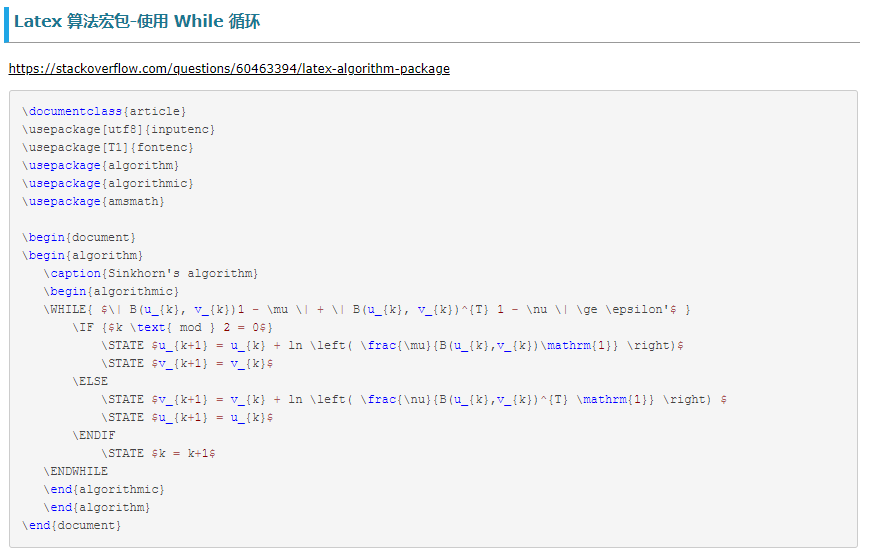
\includegraphics[scale=.6]{./pics/TeX编程搜索结果.png}
    \caption{\TeX{}编程搜索结果}
    \label{TeX编程搜索结果}
\end{figure}

这个就是教你怎么写伪代码的帖子,并不是教你像C那样使用\TeX{}进行宏编程\Footnote{详细的,系统的教程必然只能你自己去看TeXByTopic, %
TheTexbook这类的书学习。学完后建议总结一下分享在博客,扩大\TeX{}的影响力,促进知识平等}的教程。
我当初就是没能找到合适的帖子\Footnote{你可以在LaTeXStudio的官网中找到宏编程这个栏目,但是由于我是白嫖党,%
自然我会为了发扬白嫖精神,写这篇教程[doge]},
可能也是因为我不会使用\cmd{Chrome}吧。所以才用了今天的这篇文章,并不是那么系统的介绍{\bf 宏编程}的文章。

其实你也可以认为我的这篇文章就是一个为了类比主流语法的{\bf 缝合怪},我并不会说什么。因为我是按照目前主流的\cmd{C, C++, Python}的
{\bf 编程范式}来组织这篇文章的,并没有按照其他的例如\cmd{HasKell, Mathematica}这种函数式编程范式风格组织的。


\subsection{变量定义}
其实就是用一个符号去代表某个值,我们可以使用如下的几个命令:
% \Cmd{\let,\def,\gdef,\newcommand,\NewDocumentCommand}
\begin{multicols}{2}
    \begin{itemize}
        \item \cmd{def}:定义
        \item \cmd{gdef}:全局定义
        \item \cmd{let}:命令的重命名复制
        \item \cmd{newcommand}:最常用的定义方式
        \item \cmd{NewDocumentCommand}:xparse\kern-.1em\hbox{宏包提供}
    \end{itemize}     
\end{multicols}

比如我使用\cmd{sex}表示性别,定义一个变量\Footnote{注意:和主流编程语言不同的是,在\LaTeX{}中,变量均为以\cmd{\ }开头}%
\cmd{sex=female}.

\vspace*{1em}
\def \sex {female}
\fbox{
    \parbox{10em}{
        \Cmd{\def\sex{female}}
        \cmd{\sex}
    }
}
\result{10cm}
\fbox{
    \parbox{2.5em}{
        \sex
    }
}


\subsection{函数定义}
\subsubsection{格式控制函数}
类比C语言里面的函数,无非就是输入一些参数,然后给你返回一些参数,其实还是用的上面的几个宏。只不过我们这里的
函数理解为{\bf 替换}好一点,其实就是把一个命令替换为自己提前定义的内容,只不过我们可以对{\bf 替换}的内容
进行一些的格式设置。下面我们定义一个用于把以文本复制一次的命令\cmd{\copytext\{text\}},它接受一个\cmd{text}文本,然后
把这个\cmd{text}复制一次输出,把原本的\cmd{text}原样输出,复制的\cmd{text}输出颜色为橙色。

\vspace*{1em}
\def \copytext#1 {#1\textcolor{orange}{#1}}
\fbox{
    \parbox{15em}{
        \cmd{\def}\cmd{\copytext\#1\{\%}\\%
        \hspace*{2em}{\ttfamily \#1\textbackslash{}textcolor\{orange\}\{\#1\}\}}\\
        \cmd{\copytext\{Test\}}
    }
}
\result{12cm}
\fbox{
    \parbox{4em}{
        \copytext{Test}
    }
}

\vspace*{1em}
其实{\LaTeX}中环境的定义就是命令\cmd{\def}的一种拓展而且,无非就是在一个段落的前面和后面
加了一个\cmd{前置定义}和\cmd{后置定义},这个没什么好说的。

\subsubsection{数值计算函数}
由于\TeX{}这玩意儿的计算能力本来就不咋行,在无数个文档中见过这个了([doge]).所以如果你想要
自定义一些进行数值运算的函数的话,恐怕就得使用\cmd{xfp}这个宏包,这个宏包的使用方法是十分的】
简单的,官方文档也就几页,10min保证就会用了。然后你就可以用它来定义一些内容了。

但是如果你不只是仅仅拘泥于\TeX{}这个玩意儿用于计算的话,那么你的选择就太多了,
你可以使用外部语言\cmd{Lua}, \cmd{Python}, \cmd{GNUPlot}的计算能力。
你甚至还可以使用\cmd{Mathematica},要使用\cmd{Mathematica}你只需要安装一个Mathematica的云还是啥的,
在加上一个别人开发的\cmd{latexalpha2}宏包,你就可以使用\cmd{Mathematica}的符号计算,绘图,表格
等几乎所有功能。然而这一切的一切都只需要你在编译\cmd{TeX}源文件的时候开启\Cmd{--shell-escape}参数即可。
最后,最麻烦的不过就是多编译几次的问题,但是这个编译次数的问题也可以通过\cmd{latexmk}脚本完成。


最后在提一句,其实在tikz绘图中,我们很多时候都需要通过计算两个坐标,从而得到目标坐标。
而tikz中使用的是\cmd{calu}库,使用的语法就像是下下面这样的:
\begin{lstlisting}
\draw[->] (0, 0)--($(a, b) + (c, d)$);
\end{lstlisting}

所以亦可以把\cmd{calu}库看作是定义好的函数库,只不过我们的调用格式\Footnote{我们自然也可以在tikz的坐标运算中使用xfp库}不同罢了。


\subsection{流程控制}
\subsubsection{条件判断函数}
由于\LaTeX{}没有现代的{\bf 变量系统}的概念,所以对于不同类型的变量我们需要使用不同的判断函数,
但是有一个好处,它们都是类似的。下面举例常用的判断函数:
\begin{itemize}
    \item \cmd{\ifx}:比较两个宏或控制序列是否具有相同的定义
    \item \cmd{\ifmmode}: 是否在数学模式(环境)
    \item \cmd{\ifvmode}: 是否在竖直模式
    \item \cmd{\ifhmode}: 是否在水平模式
    \item \cmd{\ifinner}: 是否在内部模式,内部模式包括数学模式和文本模式,与竖直模式和水平模式不同
    \item \cmd{\ifnum}:对两个数值进行比较,\cmd{\countA}<\cmd{\countB}
    \item \cmd{\ifdim}:对两个长度进行比较,\cmd{\ifdim}\cmd{\dimA}<\cmd{\dimB}
    \item \cmd{\ifodd}:检查一个数是否为奇数,\cmd{\ifodd}\cmd{\countA}
    \item \cmd{\ifempty}:检查一个宏是否为空,\cmd{\ifempty}\cmd{\foo}
\end{itemize}

这些判函数可以与条件语句(如 \cmd{\if}、\cmd{\else}、\cmd{\fi})结合使用,用于根据条件执行不同的代码块.
下面以\cmd{\ifodd}举例:


\vspace*{1em}
\def\numA{23}
\fbox{
    \parbox{17em}{
        \cmd{\def}\cmd{\numA\{23\}}\\
        {\ttfamily\%}\Cmd{前面一个{}用于说明语句结束}\\
        {\ttfamily\% 前一个\{\}也可以使用\cmd{\relax}替代}\\
        \Cmd{\ifodd\numA}\\
        \hspace*{2em}\Cmd{{}}\cmd{\numA}\Cmd{{}}\quad\cmd{Is Odd}\\
        \Cmd{\else}\\
        \hspace*{2em}\Cmd{{}}\cmd{\numA}\Cmd{{}}\quad\cmd{Is Evan}\\
        \Cmd{\fi}
    }
}
\result{13cm}
\fbox{
    \parbox{8em}{
        \ifodd\numA
            % 前面一个{}用于说明语句结束
            {}\numA{} Is Odd
        \else
            {}\numA{} Is Evan 
        \fi
    }
}

\subsubsection{流程控制语句}
需要注意的是\LaTeX{} 中是没有类似于C语言里面的逻辑运算符号\Cmd{||, &, !, <=, >=},所以想要进行这些操作就只能
我们写一个多重判断了\Footnote{当然,如果你使用\LaTeX3的话,语法会更加的简洁,包括下面的循环也是一样的},其实就是多个单一判断的嵌套
\Footnote{在\LaTeX{}中使用判断时:{\bf 每一层}判断只能有一个\cmd{\else}}。

$\bullet$ 比如我们要判断 $2<x<5$,那么我们就需要向下面这么写:

\begin{lstlisting}
\ifnum \x>2 \ifnum \x<5
    % 符合2<x<5时进行的操作
\fi\fi
\end{lstlisting}

$\bullet$ 进一步,为了使用下面的这个$\le$功能,我们可以使用类似如下的代码实现

% \clearpage
\begin{lstlisting}
\def\numA{12}
\def\numB{15}

\ifnum\numA<\numB\relax
    \numA<\numB
\else 
    \ifnum\numA=\numB\relax
        \numA=\numB
    \else
        \numA>\numB
    \fi
\fi
\end{lstlisting}

实际效果演示:
\def\numA{12}
\def\numB{15}
\ifnum\numA<\numB\relax
    \numA<\numB
\else 
    \ifnum\numA=\numB\relax
        \numA=\numB
    \else
        \numA>\numB
    \fi
\fi


\subsection{循环}
其实接触过\LaTeX{}的TiKZ选手应该都知道里面有一个\cmd{\foreach}循环,、
这个东西可以用来绘制一些比较复杂的图形。那么假如不在绘图的\cmd{tikzpicture}
环境中使用\cmd{\foreach}循环呢?可行吗? --- {\bf 可行的}.

\subsubsection{小型循环}
下面就是一个简单的演示,演示了怎么遍历一个有限的,或者是说比较短的列表
\begin{lstlisting}
\def\list{
    1, 2, 3, 4, 5, 6, 7, 8, 9    
}
\foreach \num in \list{
    \num
    % 当num=5时换行
    \ifnum\num=5
        \par
    \fi
}
\end{lstlisting}

\def\list{
    1, 2, 3, 4, 5, 6, 7, 8, 9    
}
\foreach \num in \list{
    \cmd{\num} = \num
    % 当num=5时换行 
    \ifnum\num=5
        \par
    \fi
}

肯定有人想说,你的这个列表这么的短,有必要用循环吗?的确,假如一个列表很短,是没有必要使用循环的。
但是我们假如想要进行比较长的列表的遍历,或者说是很长的列表的遍历,比如一个拥有999个元素的列表,
我们自然希望有类似C语言的那种简洁的写法 \Cmd{\for{i=1; i<=1000; i++}{...}}

\subsubsection{大型循环}
其实\LaTeX{}给我们提供了一个语法糖来达到列表的构建目的。\Cmd{{1,2,...,100}},这个语法
其实就是表示我们要创建一个$1,2,3,...,100$这样的从1到100的列表,而不用自己一个一个的写出来。

\clearpage

下面我们把$0\circ\sim 30^\circ$之间的所有正弦值统统计算出来。\Footnote{注意:由于要计算这种复杂的函数值,
所以我使用了一个\cmd{xfp}宏包。}这个时候你应该不会想不开自己去计算吧,但是你其实可以在调用外部程序,比如GNUPlot
去计算,然后插入。亦或者是直接在类似于Matlab或者是Python中算出来,保存为\cmd{txt}格式,
然后自己到\cmd{tablegenrator}生成表格\cmd{TeX}源码,然后你把源码复制进来,微调一下编译。
下面我们使用循环生成数据:

\vspace*{1em}
% \noindent\rule{1\linewidth}{1pt}

\begin{lstlisting}
%\usepackage{xfp}
\foreach \Angle in {1,2,...,30}{
    $\sin(\Angle^\circ)$ = \fpeval{sin(deg(\Angle))}
}
\end{lstlisting}


\noindent\phantom{\hspace*{-.4em}} % 这个幻影空格用于对齐操作
\foreach \Angle in {1,2,...,30}{
    $\sin(\Angle^\circ)$ = \fpeval{sin(deg(\Angle))}
}


\subsubsection{死循环}
目前能够实现死循环的方法,很简单,直接让\TeX{}的模式切换混乱就行了\textcolor{red}{\bf (千万不要执行此操作,除非你明确你自己在干什么)}。
具体见下面的代码\Footnote{代码来源:\Cmd{https://liam.page/2020/04/28/hhh-explodes-TeX/}}
\begin{lstlisting}
\def\par{}
x\vskip 1pt
\end{lstlisting}


\subsubsection{递归}
由于\LaTeX{}中没有类似与C中那样的\cmd{while}循环,自然也就没有对应的那种\cmd{break}语句。
但是你可以在\LaTeX{}中使用{\bf 递归}。对,就是{\bf 递归},就是那个萌新最爱的递归。


我们定义了一个递归函数\Footnote{但是这里其实并不是严格的递归,有一点\Cmd{while ... break}的感觉}%
\cmd{\myLoop},它接受一个参数\cmd{#1}表示循环的次数。
在函数体中,我们首先进行条件判断,如果\cmd{#1}大于0,则执行循环体代码,
并通过递归调用\cmd{\myLoop}{\ttfamily\textbackslash numexpr\#1-1\cmd{\relax}} 来实现循环。
递归调用中的参数是\cmd{#1} 减去1,即实现了循环次数的递减.然后我们调用\cmd{\myLoop\{5\}} 来执行循环,
输出了着5次循环中的迭代信息

\begin{lstlisting}
\newcounter{myLoopCounter}
\newcommand{\myLoop}[1]{%
    \setcounter{myLoopCounter}{#1}%
    \loop
        \ifnum\value{myLoopCounter}>0
        % 循环体代码
        Loop iteration: \the\value{myLoopCounter}\par
        \addtocounter{myLoopCounter}{-1} % 计数器减1
    \repeat
}

\myLoop{5}
\end{lstlisting}


\newcounter{myLoopCounter}
\newcommand{\myLoop}[1]{%
    \setcounter{myLoopCounter}{#1}%
    \loop
        \ifnum\value{myLoopCounter}>0
        % 循环体代码
        Loop iteration: \the\value{myLoopCounter}\par
        \addtocounter{myLoopCounter}{-1} % 计数器减1
    \repeat
}


\myLoop{5}


其实\LaTeX3{}里面的这个代码才算真正的递归(只是代码片段,不完整)
\begin{lstlisting}
\cs_set:Npn \fibon:n #1{
    \int_compare:nNnTF{#1}={0}{0}
    {
        \int_compare:nNnTF{#1}={1}{1}
        {
            \fp_eval:n{\fibon:n{#1-1}+\fibon:n{#1-2}}
        }
    }
}
\end{lstlisting}


\subsection{数据结构}

\subsubsection{结构体}
其实我们可以仿照C语言中结构体的定义,自己创建一个{\bf 结构体}对象,然后给它关联一些的属性,
从而进一步实现C语言中的各种复杂的数据结构。这里的难点在于你要怎么关联对应的属性

\subsubsection{链表}
只要结构体能够实现,那么这个链表的实现也是比较简单的,只不过要找到一个类似于
指针的东西 ??






\end{document}

%%%%  尝试在自定义宏中执行catcode的测试代码
% \documentclass{article}
% \usepackage{xparse}
% \usepackage{ctex}

% \def\cmdb{|catcode\`{}\=0}
% \NewDocumentCommand{\cmda}{m}{%
%     \catcode`|=0
%     \catcode`\\=12
%     {\ttfamily \scantokens{#1}}  
% }
% \def\cmdc{\string|LaTeX}


% \def\cmd#1{\cmda{#1}\cmdb}


% \begin{document}
% 调用命令的结果:\cmda{\def} |LaTeX


% 测试原始的\textbackslash{}的catcode有没有改正回来: \LaTeX

% |catcode`\=0
% 测试原始的\textbackslash{}的catcode有没有改正回来: \LaTeX

% \cmd{\h}

% |cmdc

% |end{document}



